\documentclass[tikz,border=2pt]{standalone}
\usepackage{amsmath}
\usepackage{pgfplots}
\pgfplotsset{compat=1.18}
\usetikzlibrary{arrows.meta}
\begin{document}
% Example 1: max 3x1+2x2 s.t. x1+x2<=4, -x1<=-1 (x1>=1); feasible region with corners (1,0),(4,0),(1,3).
% Big-M path: start (0,0) with w=1, Z=-M (infeasible for the LP) -> x1 enters, w leaves -> (1,0), Z=3
% -> s2 enters, s1 leaves -> (4,0), Z=12 optimal.
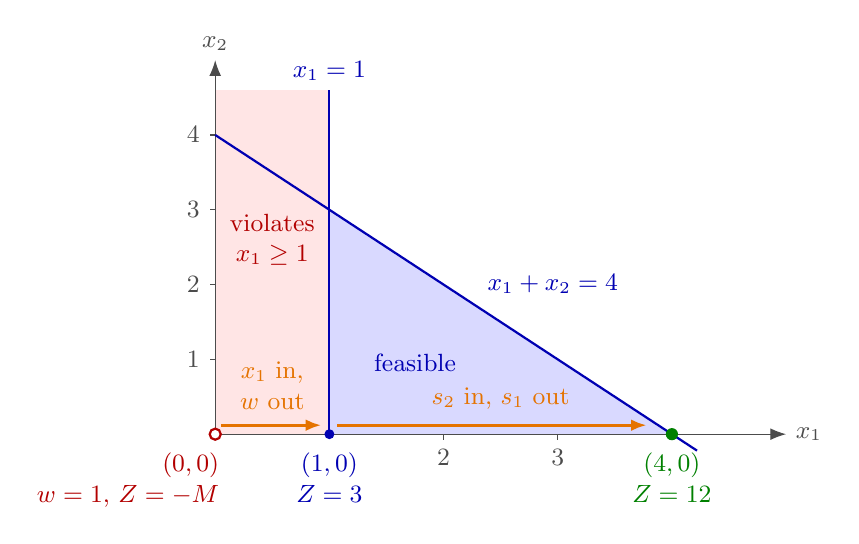
\begin{tikzpicture}[font=\small, >={Latex[length=2mm]}, x=1.45cm, y=0.95cm]
  \fill[red!10] (0,0) rectangle (1,4.6);
  \fill[blue!15] (1,0) -- (4,0) -- (1,3) -- cycle;
  \draw[->, gray!60!black] (0,0) -- (5,0) node[anchor=west] {$x_1$};
  \draw[->, gray!60!black] (0,0) -- (0,5) node[anchor=south] {$x_2$};
  \foreach \x in {2,3} \draw[gray!60!black] (\x,0) -- (\x,-0.08) node[anchor=north] {$\x$};
  \foreach \y in {1,2,3,4} \draw[gray!60!black] (0,\y) -- (-0.05,\y) node[anchor=east] {$\y$};
  \draw[blue!70!black, thick] (1,4.6) -- (1,0);
  \draw[blue!70!black, thick] (0,4) -- (4.22,-0.22);
  \node[blue!70!black, anchor=south] at (1,4.6) {$x_1=1$};
  \node[blue!70!black, anchor=south west] at (2.3,1.75) {$x_1+x_2=4$};
  \node[red!70!black, align=center] at (0.5,2.6) {violates\\ $x_1\geq1$};
  % path
  \draw[->, orange!90!black, very thick] (0.05,0.12) -- (0.93,0.12);
  \draw[->, orange!90!black, very thick] (1.07,0.12) -- (3.78,0.12);
  \node[orange!90!black, align=center, anchor=south] at (0.5,0.2) {$x_1$ in,\\ $w$ out};
  \node[orange!90!black, anchor=south] at (2.5,0.2) {$s_2$ in, $s_1$ out};
  % points
  \draw[red!70!black, thick, fill=white] (0,0) circle (2pt);
  \fill[blue!70!black] (1,0) circle (1.8pt);
  \fill[green!50!black] (4,0) circle (2.2pt);
  \node[red!70!black, anchor=north east, align=right] at (0.12,-0.12) {$(0,0)$\\ $w=1$, $Z=-M$};
  \node[blue!70!black, anchor=north, align=center] at (1,-0.12) {$(1,0)$\\ $Z=3$};
  \node[green!50!black, anchor=north, align=center] at (4,-0.12) {$(4,0)$\\ $Z=12$};
  \node[blue!70!black] at (1.75,0.95) {feasible};
\end{tikzpicture}
\end{document}
